%
% $RCSfile$
%
% Copyright (c) 2005-2006. Christian Heller. All rights reserved.
%
% Permission is granted to copy, distribute and/or modify this document
% under the terms of the GNU Free Documentation License, Version 1.1 or
% any later version published by the Free Software Foundation; with no
% Invariant Sections, with no Front-Cover Texts and with no Back-Cover
% Texts. A copy of the license is included in the section entitled
% "GNU Free Documentation License".
%
% http://www.cybop.net
% - Cybernetics Oriented Programming -
%
% http://www.resmedicinae.org
% - Information in Medicine -
%
% Version: $Revision$ $Date$ $Author$
% Authors: Christian Heller <christian.heller@tuxtax.de>
%

\subsection{Abstraction Gaps}
\label{abstraction_gaps_heading}

Software has to be developed in a creative process called
\emph{Software Engineering Process} (SEP) or \emph{Methodology} (figure
\ref{gaps_figure}).

\begin{figure}[htb]
    \begin{center}
        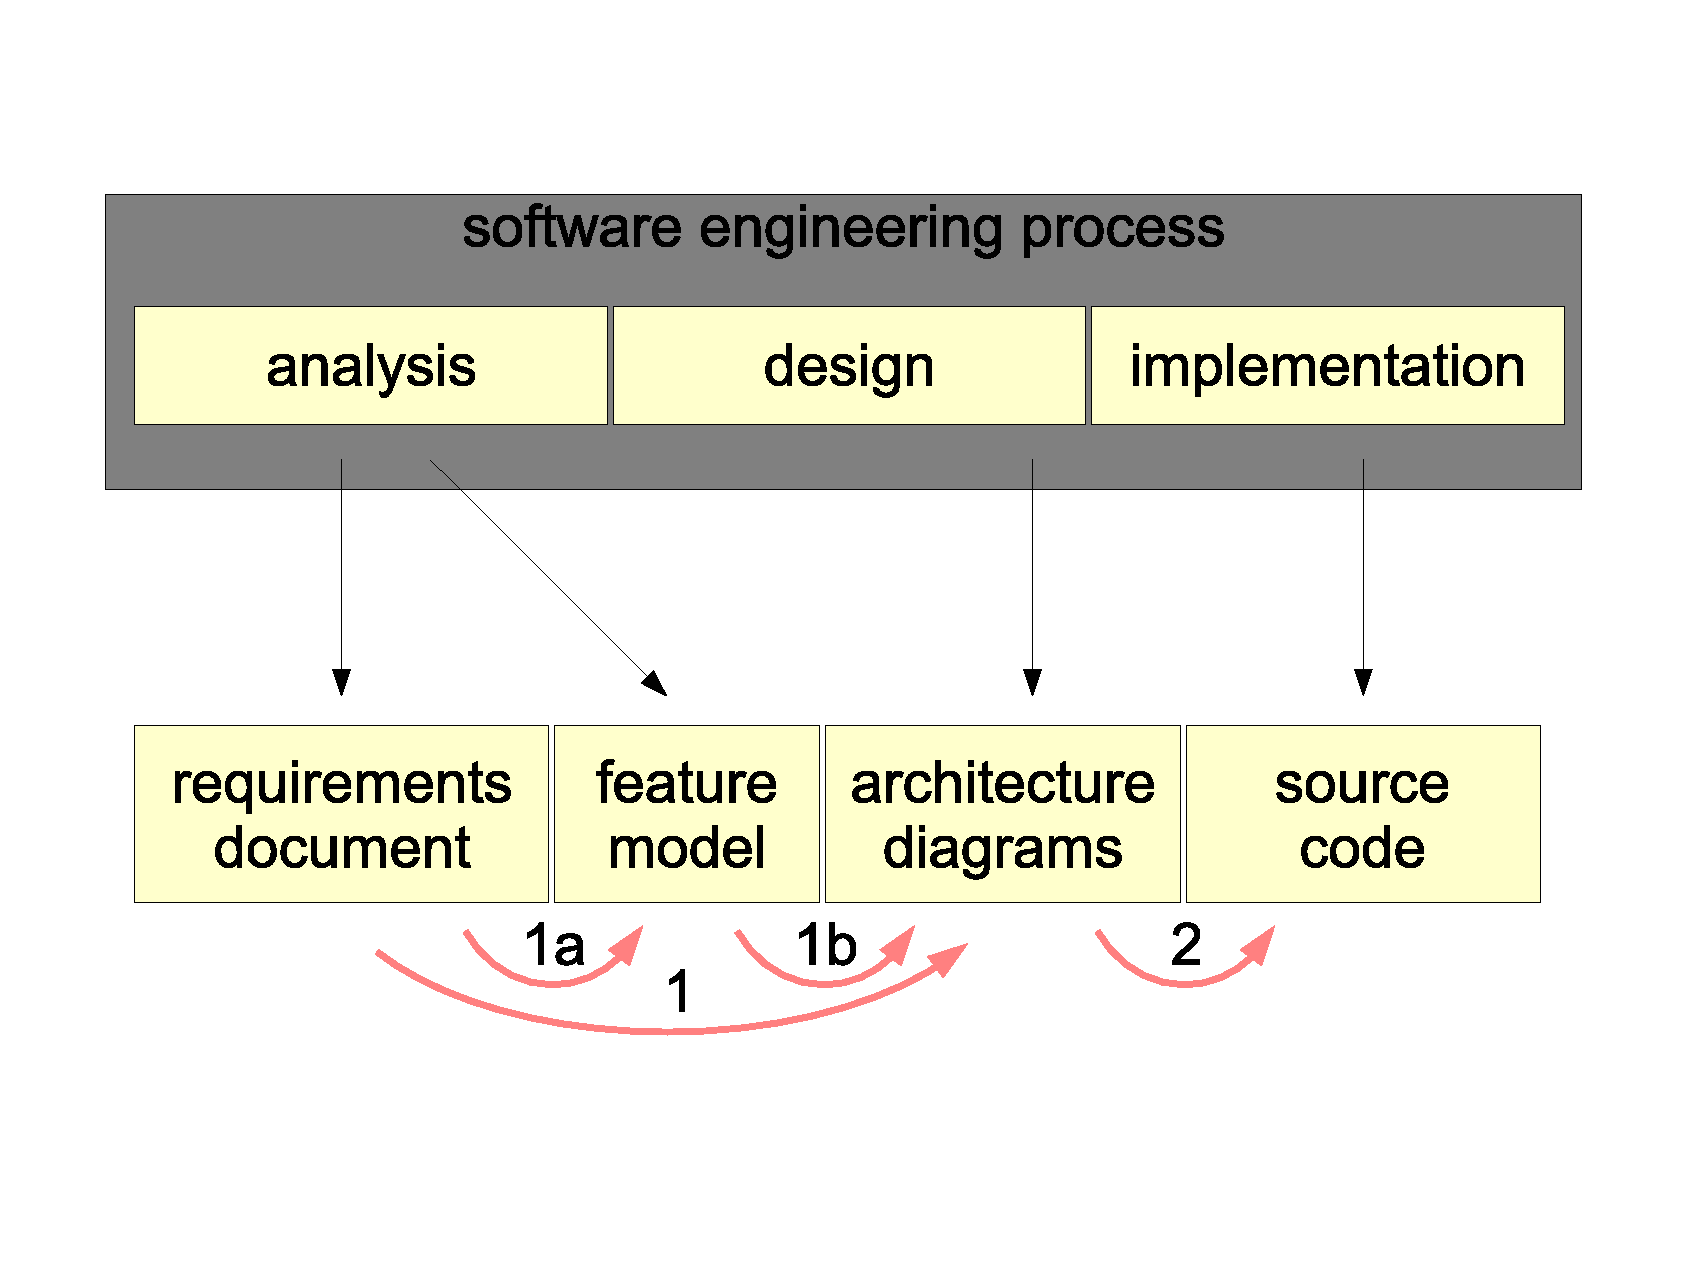
\includegraphics[scale=0.2]{vector/gaps.eps}
        \caption{Abstraction Gaps}
        \label{gaps_figure}
    \end{center}
\end{figure}

Different forms of SEP exist: \emph{Waterfall}, \emph{Iterative},
\emph{Extreme Programming} (XP) and \emph{Agile Programming}. But every
project, consciously or not, follows a SEP that sooner-or-later, in one form or
the other, goes through three common phases: \emph{Analysis}, \emph{Design} and
\emph{Implementation}. Each phase creates its own model of what is to be
abstracted in software and it is the differences in exactly these models that
often cause complications.

A previous article \cite{heller2004} mentioned the \emph{Requirements Document},
\emph{Feature Model}, \emph{Architecture Diagrams} and \emph{Source Code} as
forms of knowledge abstraction. It also described the following abstraction
gaps (see figure \ref{gaps_figure}) that have to be crossed:

\begin{enumerate}
    \item[1a] Requirements Document/Feature M.
    \item[1b] Feature Model/Architecture Diagr.
    \item[2] Architecture Diagrams/Source Code
\end{enumerate}

By improving the \emph{Traceability} between requirements and the architecture,
feature models (known from system family/ product line engineering) contribute
to minimising gap 1. Together with architecture diagrams, they ease
communication between stakeholders in the SEP, because of their human-readable
form and implementation-independence. But sooner-or-later, also these have to
be transferred into source code, by crossing gap 2.

Bridging or closing these abstraction gaps (sometimes called \emph{Semantic- or
Conceptual Gaps}) is also known as: \textit{achieving higher intentionality}
and remains an unsolved task for software engineering. One aim of the work
described in this article was to contribute to a possible solution, with focus
on \emph{reducing} gap 2, existing between a designed architecture and the
implemented code.
